\chapter{Der Kobold Client}
Der Client basiert grundlegend auf der Eclipse Plattform und deren Widgettoolkit und ist
dadurch von dessen nativer Schnittstelle abh�ngig. 
Er wird als "Feature-Set" implementiert und mit "Product Branding" versehen.
"Product Branding" umfasst die �nderung der Fensternamen und der Produktsymbole, sowie
einer Willkommensseite, die einen kurzen �berblick �ber Funktionalit�t und Zweck des Kobold Tools geben soll.

Das Feature-Set wird als Set von internationalisierbaren Eclipse Plugins implementiert.
Die Ausgangsperspektive besteht aus 4 Teilen:
\begin{itemize}
	\item Der Produktlinienarchitektur Editor
	\item Die Rollen View
	\item Die Worklflow/Task View
	\item Die Minimap
\end{itemize}
Diese werden in den jeweiligen Unterkapiteln n�her beschrieben.
Um das Rollenprinzip konsistent durchzusetzen, ist eine zentrale Anmeldung an dem Kobold Serverdienst n�tig.
Details zu der serverseitigen L�sung finden Sie in Kapitel 5.

 \begin{figure}[ht]
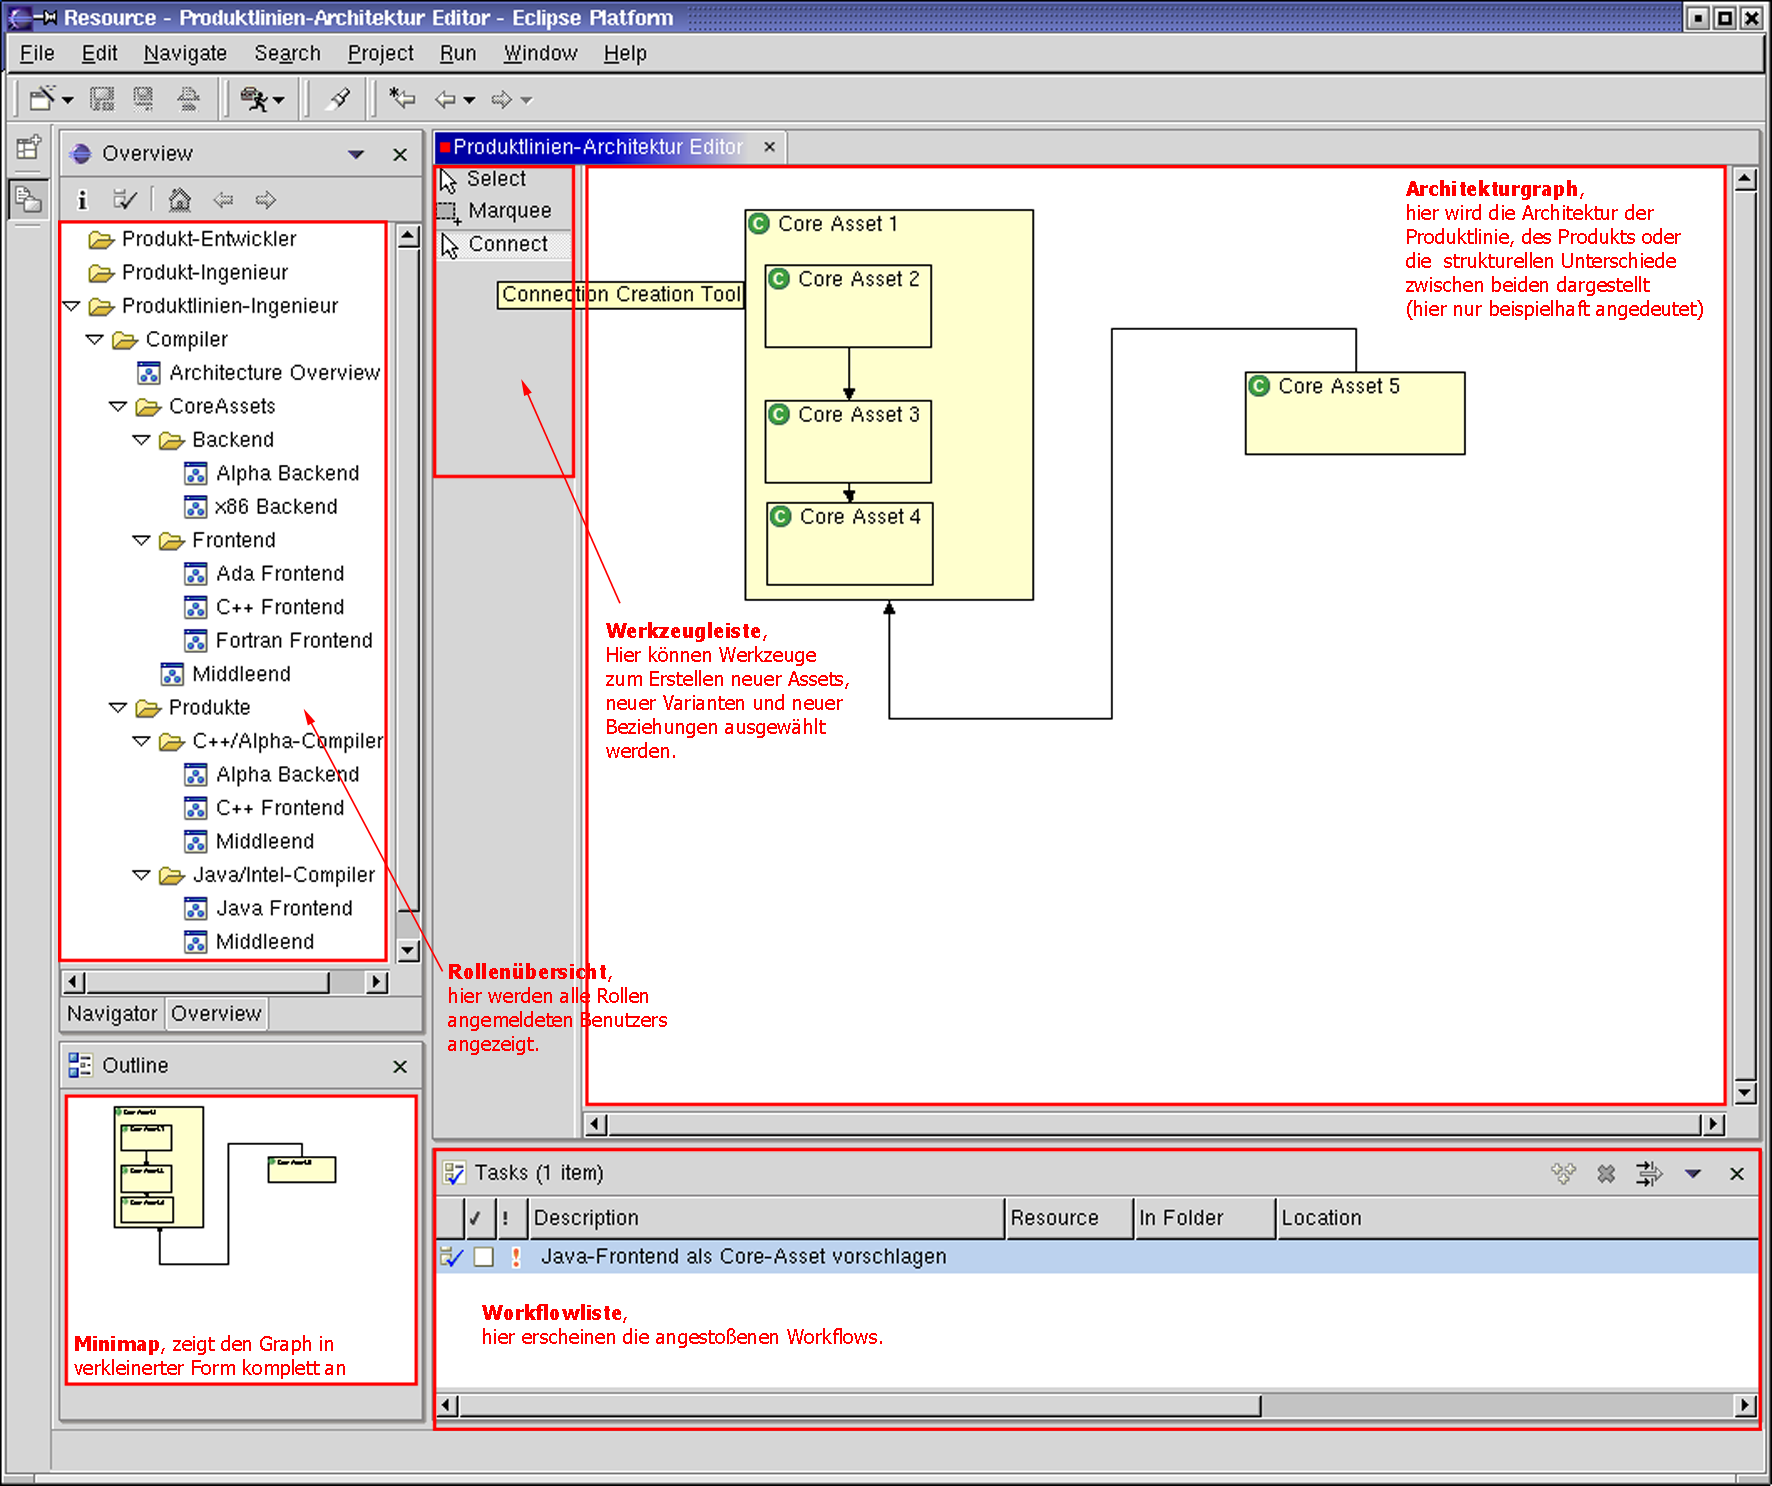
\includegraphics[width=15cm]{../angebot/screenshot.png}
   \caption{Screenshot des Client-Prototypen}
\end{figure}

\section{Authentifizierung}
Die Authentifizierung am Server erfolgt durch RPC. Der Benutzer kann bei der Erstbenutzung des 
Clients w�hlen, ob er sich bei jedem Programmstart authentifiziern will oder ob das Passwort
und der Benutzername gespeichert werden sollen. Prinzipiell ist ein �ndern von Daten im nichtauthentifizierten
Zustand nicht m�glich. Mit der Authentifizierung werden die Rollen, die dem Benutzer zugeteilt sind,
an den Client �bergeben; der Client reagiert seinerseits mit dem Bereitstellen der relevanten Views f�r den Benutzer.

\section{Der Produktlinienarchitektur Editor}
In diesem View wird die je nach aktiver Rolle relevante Ansicht auf die Architektur der Produktlinie
angezeigt. Die grafische Notation orientiert sich dabei an der in dem Paper \cite{paper} festgelegten Struktur.
Um dies grafisch darzustellen, hier noch einmal die 3 verschiedenen Ansichten auf die
Produktlinien- bzw. Produktarchitektur.
Die Ansicht bietet die M�glichkeit, verschiedene Zoomstufen einzustellen. Eine m�gliche Folge daraus ist,
dass im aktuellen Ausschnitt m�glicherweise nicht die ganze Architektur zu sehen ist.
Um trotzdem den �berblick zu gew�hrleisten, wird eine Minimap zur Verf�gung gestellt.

\subsection{Ansicht der Rolle ProduktlinienIngenieur}
Der Produktlinieningenieur hat die M�glichkeit, zwischen zwei Ansichten zu wechseln.
Diese sind einerseits die Ansicht auf die Architektur der gesamten Produktlinie, die
sich grafisch sehr stark an der vom Paper \cite{paper} vorgeschlagenen Sicht anlehnt. Es gibt die M�glichkeit, 
bestimmte Beziehungen farblich hervorzuheben, bzw. in sp�teren Iterationen auch automatisch
hervorheben zu lassen. Grunds�tzlich kann die Farbe von Archtikturelementen gew�hlt werden. 
Einige Farben werden aber Konflikten und �hnlichen Beziehungen vorbehalten.
\begin{figure}[ht]
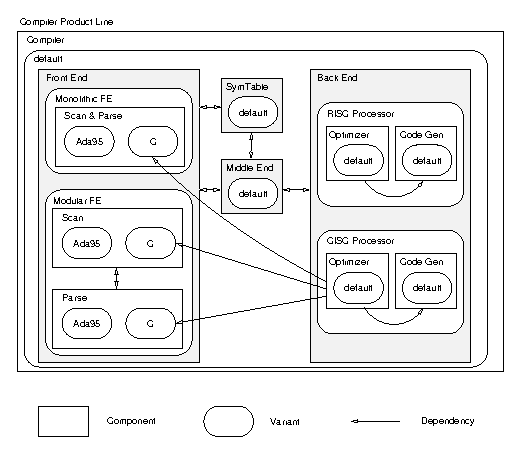
\includegraphics[width=15cm]{compiler-spl}
   \caption{Sicht des Produktlinieningenieurs}
\end{figure}
\subsection{Ansicht der Rolle eines Produktingenieurs}
Der Produktingenieur kann in dem Architektur-View immer nur ein Produkt auf einmal einsehen.
Er kann im Rollen View die verschiedenen ihm zugeordneten Produktarchitekturen der
verschiedenen Produkte zur Darstellung ausw�hlen. Grafisch wird sich Kobold hier wiederum
an der im Paper \cite{paper} orientieren.
\begin{figure}[ht]
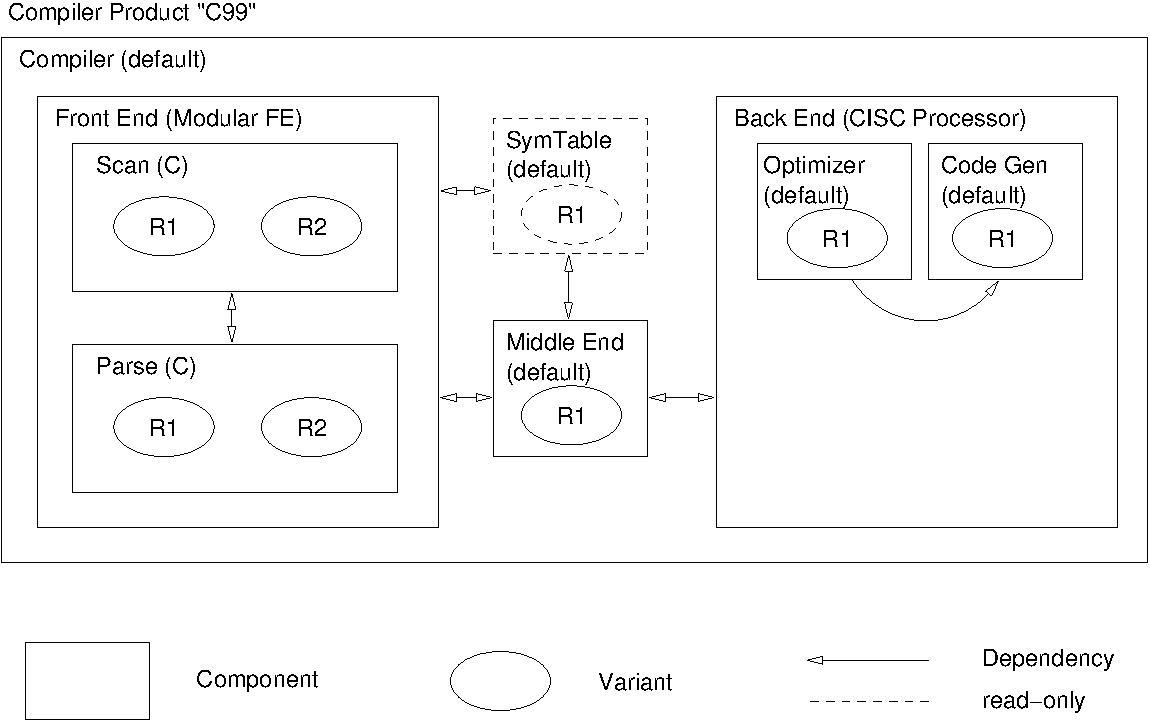
\includegraphics[width=15cm]{compiler-pe}
   \caption{Sicht des Produktingenieurs}
\end{figure}
\subsection{Ansicht der Rolle eines Programmierers}
Der Programmierer hat eine sehr flache Sicht auf ein einziges ihm zugeordnetes Produkt.
Er kann die f�r ihn �nderbaren Produktteile des Produktes von den nicht �nderbaren unterscheiden.
Es besteht die M�glichkeit, den aktuellen Stand des Produktes in seinen aktuellen "Workspace"
auszuchecken.
\begin{figure}[ht]
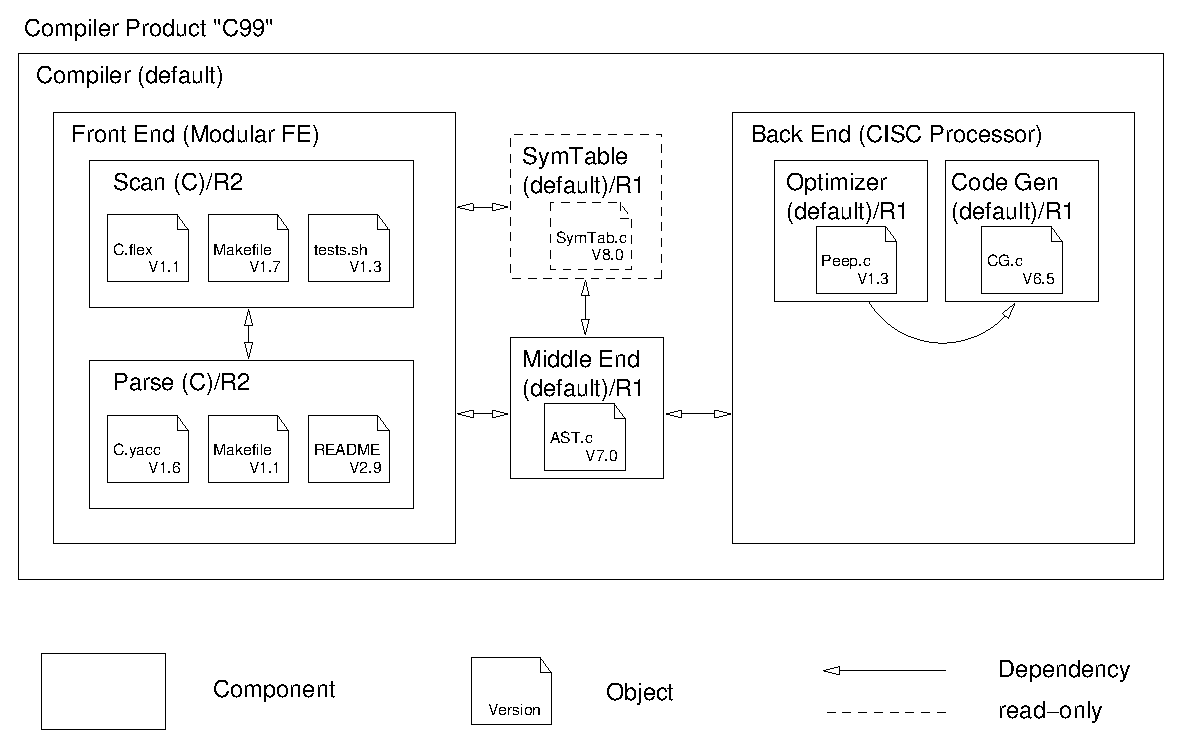
\includegraphics[width=15cm]{compiler-p}
   \caption{Sicht des Programmierers}
\end{figure}

\section{Der Rollen View}
Auf der linken Seite der Ausgangsperspektive wird ein hierarchischer Baum angezeigt, der
die momentan aktive Rolle und die mit Ihr verbundenen m�glichen Sichten darstellt.
\section{Der Worklflow/Task View}
Am unteren Rand der Ausgangsperspektive werden standardm�ssig die noch zu erf�llenden
Aufgaben, die aktuellen Nachrichten oder etwaige Konflikte und �hnliches angezeigt.

\section{Die Minimap}
Am rechten unteren Rand der Ausgangsperspektive wird eine sogennante Minimap angezeigt,
in der ein �berblick �ber die ganze Architekturansicht der aktuellen Rolle gegeben wird.



